\documentclass[aps,letterpaper,10pt]{revtex4}


\usepackage{wrapfig}
\usepackage{graphicx} % For images
\usepackage{float}    % For tables and other floats
\usepackage{verbatim} % For comments and other
\usepackage{amsmath}  % For math
\usepackage{amssymb}  % For more math
\usepackage{fullpage} % Set margins and place page numbers at bottom center
\usepackage{listings} % For source code
\usepackage{subfig}   % For subfigures
\usepackage[usenames,dvipsnames]{color} % For colors and names
\usepackage[pdftex]{hyperref}           % For hyperlinks and indexing the PDF
\usepackage[svgnames]{xcolor}
\usepackage{tikz}
\usetikzlibrary{arrows,shapes,positioning}
\tikzstyle arrowstyle=[scale=1]
\hypersetup{ % play with the different link colors here
    colorlinks,
    citecolor=blue,
    filecolor=blue,
    linkcolor=blue,
    urlcolor=blue % set to black to prevent printing blue links
}

\definecolor{mygrey}{gray}{.96} % Light Grey
\lstset{
    language=[ISO]C++,              % choose the language of the code ("language=Verilog" is popular as well)
    tabsize=3,							  % sets the size of the tabs in spaces (1 Tab is replaced with 3 spaces)
    basicstyle=\tiny,               % the size of the fonts that are used for the code
    numbers=left,                   % where to put the line-numbers
    numberstyle=\tiny,              % the size of the fonts that are used for the line-numbers
    stepnumber=2,                   % the step between two line-numbers. If it's 1 each line will be numbered
    numbersep=5pt,                  % how far the line-numbers are from the code
    backgroundcolor=\color{mygrey}, % choose the background color. You must add \usepackage{color}
    %showspaces=false,              % show spaces adding particular underscores
    %showstringspaces=false,        % underline spaces within strings
    %showtabs=false,                % show tabs within strings adding particular underscores
    frame=single,	                 % adds a frame around the code
    tabsize=3,	                    % sets default tabsize to 2 spaces
    captionpos=b,                   % sets the caption-position to bottom
    breaklines=true,                % sets automatic line breaking
    breakatwhitespace=false,        % sets if automatic breaks should only happen at whitespace
    %escapeinside={\%*}{*)},        % if you want to add a comment within your code
    commentstyle=\color{BrickRed}   % sets the comment style
}

\newcommand{\labno}{05}
\newcommand{\labtitle}{AU 332 Artificial Intelligence: Principles and Techniques}
\newcommand{\authorname}{Guowei Deng}
\newcommand{\professor}{Yue Gao}

\begin{document}

\begin{titlepage}
\begin{center}
{\Large \textsc{\labtitle} \\ \vspace{4pt}}
\rule[13pt]{\textwidth}{1pt} \\ \vspace{150pt}
{\large By: \authorname \\ \vspace{10pt}
Instructor: \professor \\ \vspace{10pt}
\today}
\end{center}
\end{titlepage}
\section{Gridworld}
\subsection{Policy iteration}
In this part, we are to implement the policy iteration for gridworld. Because the code for value 
iteration is given, the algorithm for policy iteration is not quite difficult to implement. 
Here's the result for both algorithms.\\
\begin{figure}[htbp] 
    \centering 
    \begin{minipage}[t]{0.5\linewidth}
    \centering 
    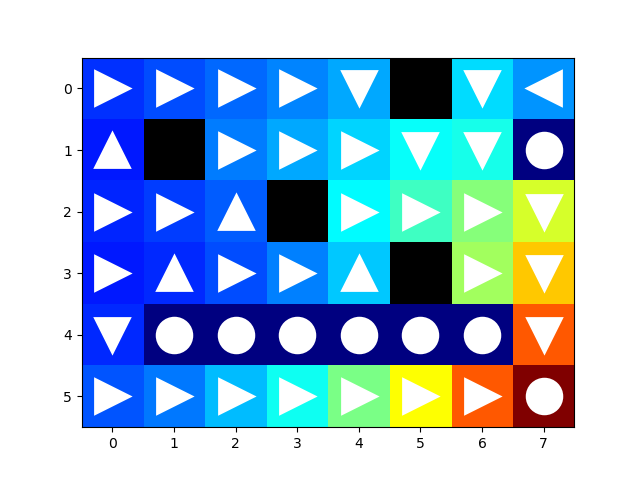
\includegraphics[scale=0.5]{value.png} 
    %\caption{fig1} 
    \end{minipage}%  
    \begin{minipage}[t]{0.5\linewidth} 
    \centering 
    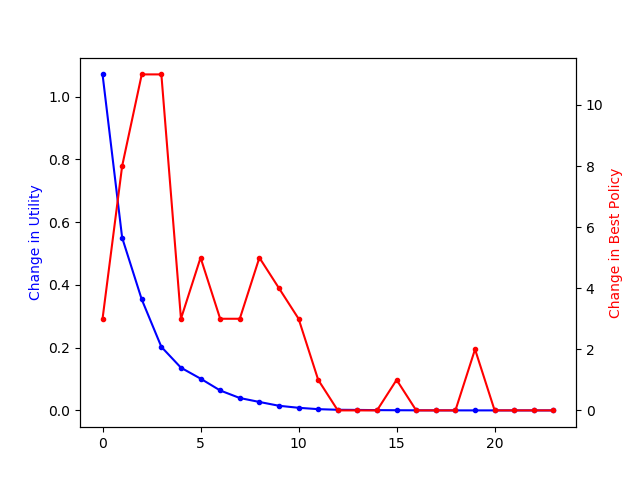
\includegraphics[scale=0.5]{value_change.png} 
    %\caption{fig2} 
    \end{minipage}% 
    \centering 
    \caption{value iteration} 
\end{figure}
\begin{figure}[htbp] 
    \centering 
    \begin{minipage}[t]{0.5\linewidth}
    \centering 
    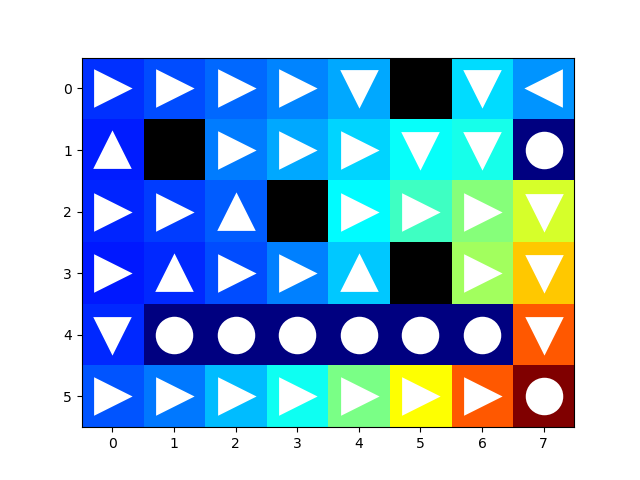
\includegraphics[scale=0.5]{Policy.png} 
    %\caption{fig1} 
    \end{minipage}%  
    \begin{minipage}[t]{0.5\linewidth} 
    \centering 
    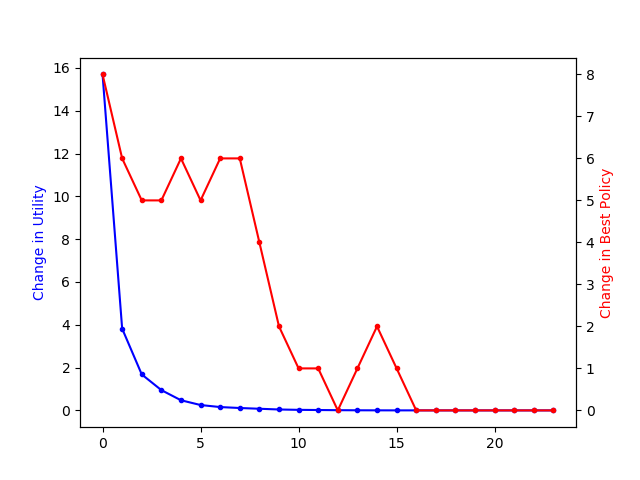
\includegraphics[scale=0.5]{Policy_change.png} 
    %\caption{fig2} 
    \end{minipage}% 
    \centering 
    \caption{policy iteration} 
\end{figure}
\par
  As we can see, both algorithms can result in optimal policy.
  But it seems that the policy iteration converges faster than 
  value iteration.
\newpage
\subsection{Qlearning and Sarsa} 
\begin{figure}[htbp] 
    \centering 
    \begin{minipage}[t]{0.5\linewidth}
    \centering 
    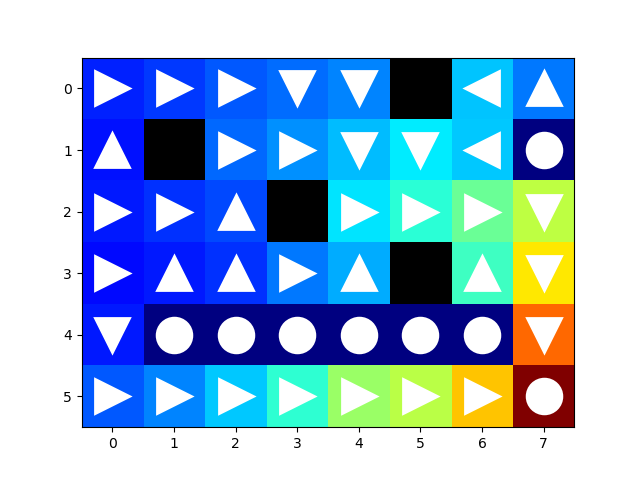
\includegraphics[scale=0.5]{ql_e_greedy.png} 
    %\caption{fig1} 
    \end{minipage}%  
    \begin{minipage}[t]{0.5\linewidth} 
    \centering 
    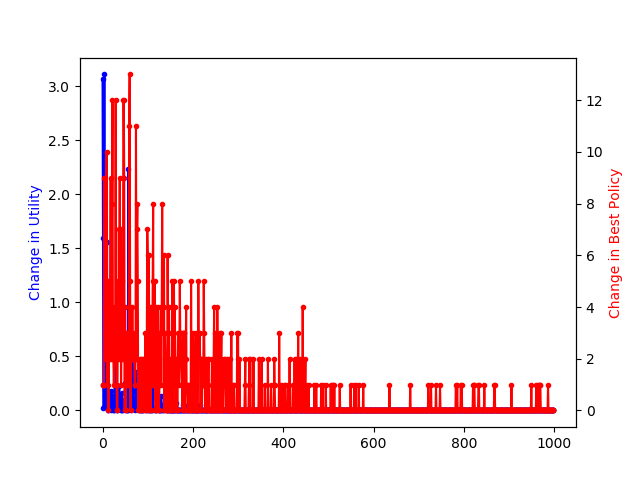
\includegraphics[scale=0.5]{ql_e_greedy_change.png} 
    %\caption{fig2} 
    \end{minipage}% 
    \centering 
    \caption{QLearning} 
\end{figure}
\begin{figure}[htbp] 
    \centering 
    \begin{minipage}[t]{0.5\linewidth}
    \centering 
    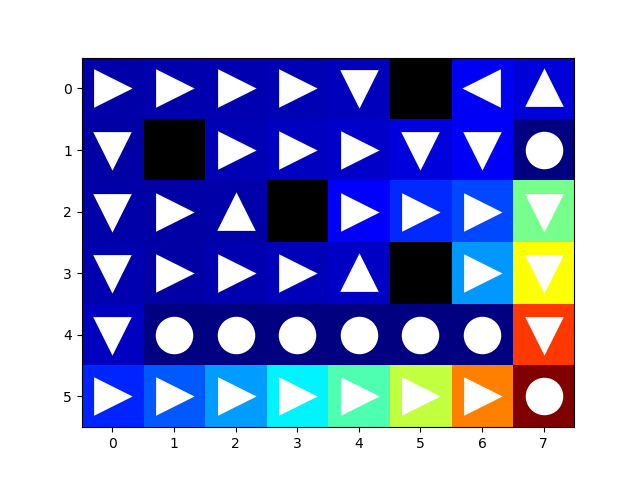
\includegraphics[scale=0.5]{sarsa_e_greedy.png} 
    %\caption{fig1} 
    \end{minipage}%  
    \begin{minipage}[t]{0.5\linewidth} 
    \centering 
    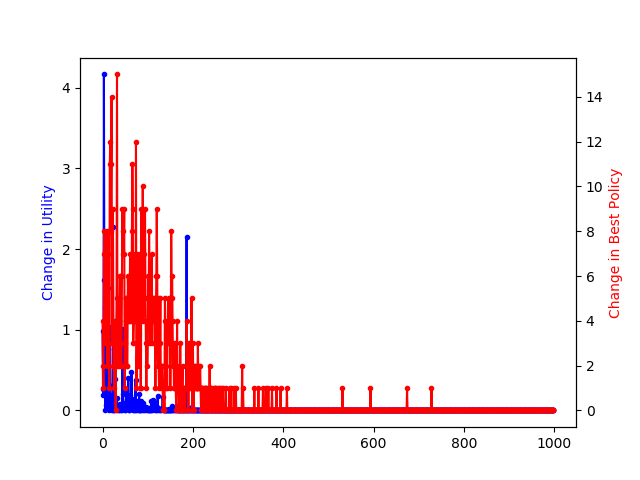
\includegraphics[scale=0.5]{sarsa_e_greedy_change.png} 
    %\caption{fig2} 
    \end{minipage}% 
    \centering 
    \caption{Sarsa} 
\end{figure}
\newpage
\subsection{Exploration function}
\par
The result for QLearning using an exploration function 
to explore is as follows:
\begin{figure}[htbp] 
    \centering 
    \begin{minipage}[t]{0.5\linewidth}
    \centering 
    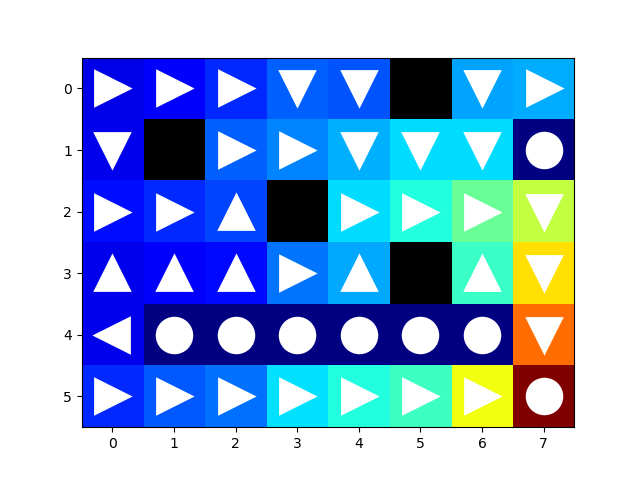
\includegraphics[scale=0.5]{ql_explore.png} 
    %\caption{fig1} 
    \end{minipage}%  
    \begin{minipage}[t]{0.5\linewidth} 
    \centering 
    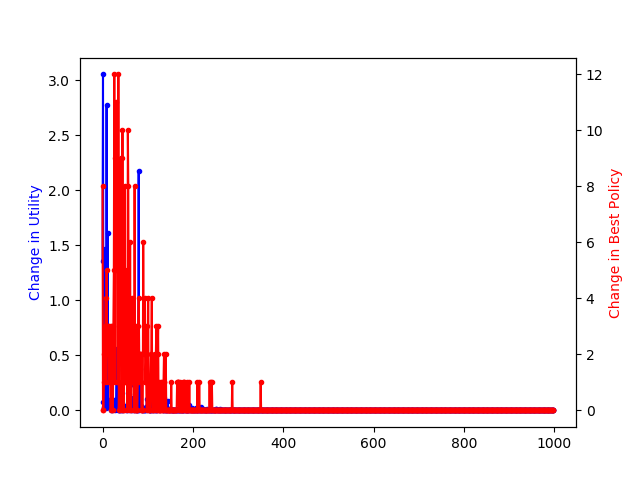
\includegraphics[scale=0.5]{ql_explore_change.png} 
    %\caption{fig2} 
    \end{minipage}% 
    \centering 
    \caption{QLearning-explore} 
\end{figure}
\par
As the graphs show briefly, there are few differences in policy 
between $\epsilon$-greedy and exploration functon. But using exploration 
function to explore, it converges much faster. The policy and Q value 
converge after only 400 iterations, while the other's policy is still 
changing after 1000 iterations. So the exploration function can reduce 
many regrets.
\newpage 
\subsection{Hyperparameters tuning}
After some thinking and trials, I finally choose hyperparameters $\alpha=0.8, \gamma=0.9, \epsilon=0.4, k=2$
    \begin{enumerate}
        \item Tuning discount rate $\gamma$:\\
        The discount rate $\gamma$ indicates how the agent evaluate the reward far 
        from it. As we can see from the policy below, if $\gamma$ is too high, then the agent will be blindly optimistic and will choose 
        a way which is closer but surrounded by traps . On the other hand, if $\gamma$ is too low, then the agent will 
        be so pessimistic and will be too scared of traps and choose the adverse direction though it 
        will stay still because of walls. 
        \begin{figure}[htbp] 
            \centering 
            \begin{minipage}[t]{0.5\linewidth}
            \centering 
            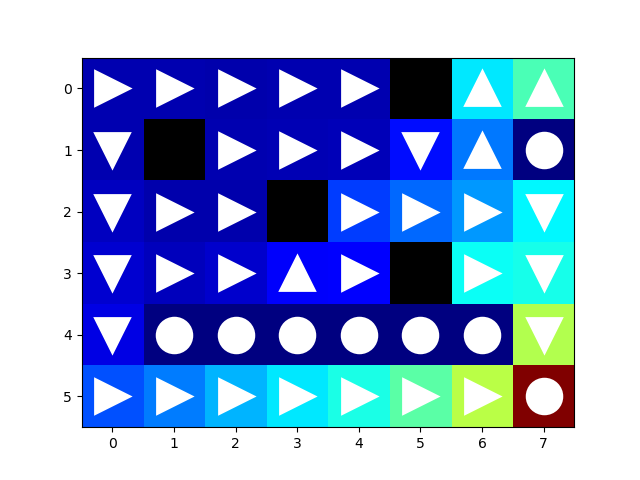
\includegraphics[scale=0.5]{sarsa_explore.png} 
            \caption{High discount} 
            \end{minipage}%  
            \begin{minipage}[t]{0.5\linewidth} 
            \centering 
            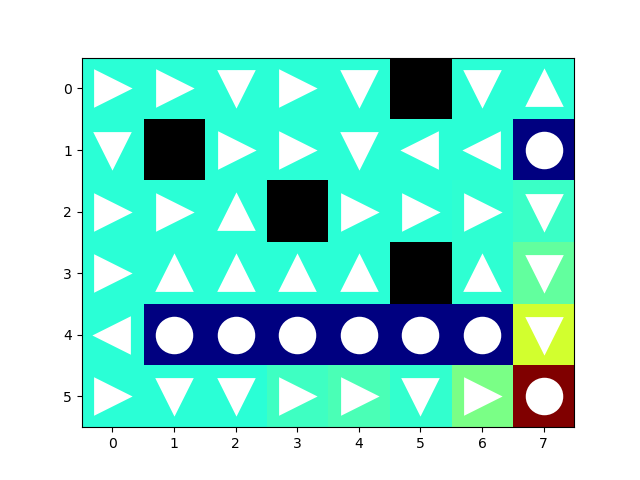
\includegraphics[scale=0.5]{low_discount.png} 
            \caption{Low discount} 
            \end{minipage}% 
            \centering 
            \caption{discount tunning} 
        \end{figure}
        \begin{figure}[htbp] 
            \centering 
            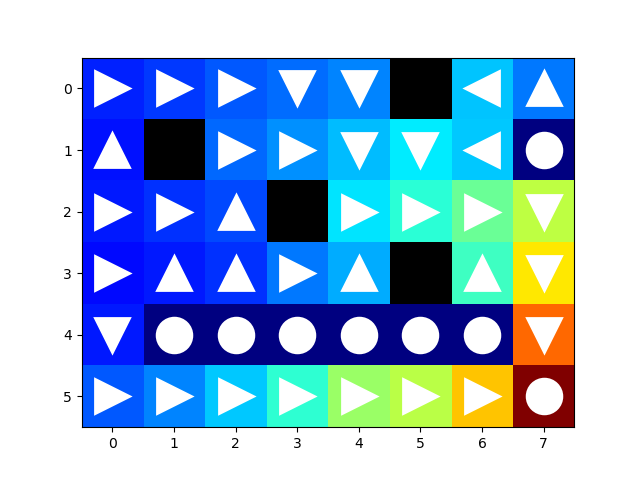
\includegraphics[scale=0.5]{ql_e_greedy.png} 
            \caption{best discount(0.9)} 
        \end{figure}
        \newpage
        \item Tuning learning rate $\alpha$:\\
        Learning rate is a quite Hyperparameter that influences 
        result of Q-learning. It indicates how much the agent will 
        give up what it has learned and how much it will accept the 
        gain it will get later. And it's quite hard to say which learning rate is better 
        before experiments. So we need to tune it from the result.\\ 
        \begin{figure}[htbp] 
            \centering 
            \begin{minipage}[t]{0.5\linewidth}
            \centering 
            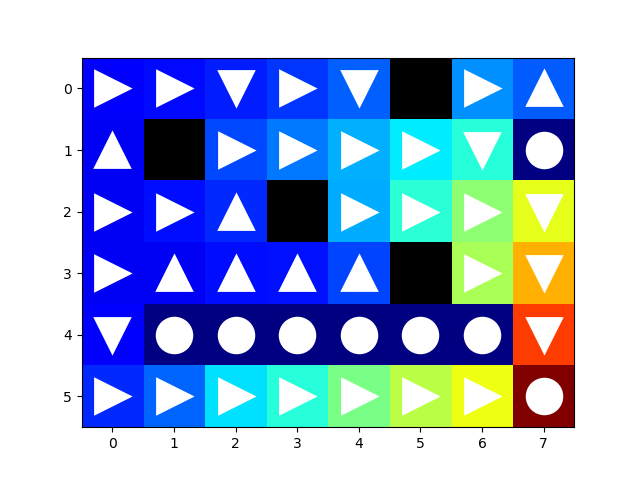
\includegraphics[scale=0.5]{a=6.png} 
            \caption{learningrate=0.6} 
            \end{minipage}%  
            \begin{minipage}[t]{0.5\linewidth} 
            \centering 
            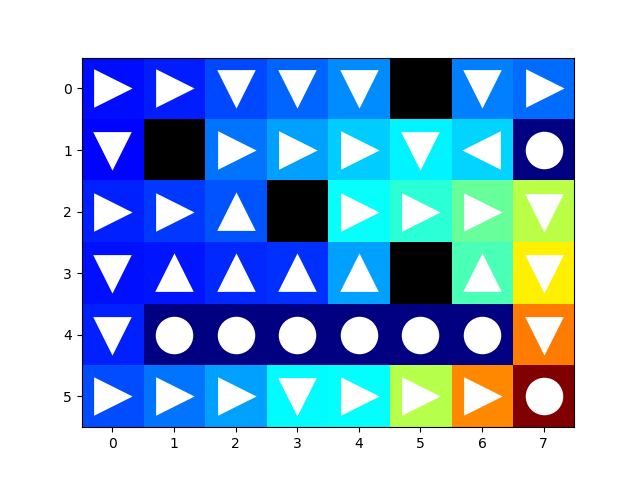
\includegraphics[scale=0.5]{a=7.png} 
            \caption{learningrate=0.7} 
            \end{minipage}%
            \\
            \centering 
            \begin{minipage}[t]{0.5\linewidth}
            \centering 
            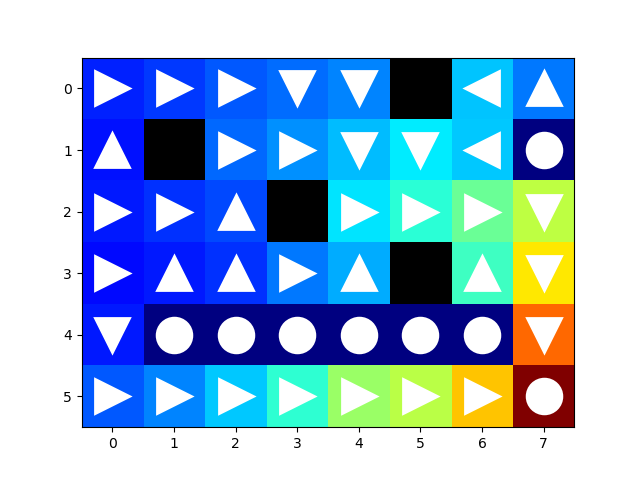
\includegraphics[scale=0.5]{ql_e_greedy.png} 
            \caption{learningrate=0.8} 
            \end{minipage}%  
            \begin{minipage}[t]{0.5\linewidth} 
            \centering 
            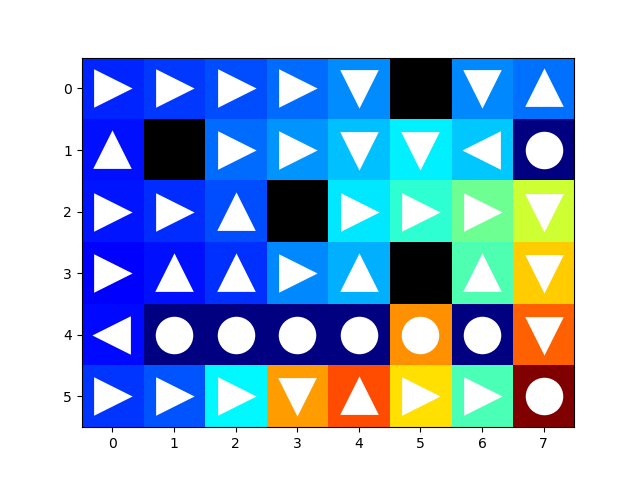
\includegraphics[scale=0.5]{a=9.png} 
            \caption{learningrate=0.9} 
            \end{minipage}%
            \centering 
            \caption{discount tunning} 
        \end{figure}
        \par
        It can be seen from the result above that if learning rate is too high, then we get 
        a quite wired result. But if learning rate is too low, some places converge to suboptimal policy. 
        And when $\alpha$ equals to 0.7 or 0.8, the result seems to be fine. 
        \newpage
        \item Tuning $\epsilon$ in $\epsilon$-greedy exploration:\\
        $\epsilon$-greedy is a method to explore the whole state space. At the very begining, agent 
        chooses action randomly to explore the world. But $\epsilon$ should decay as the agent explores 
        the world enough times. So we need to fine a proper $\epsilon$. 
        \begin{figure}[htbp] 
            \centering 
            \begin{minipage}[t]{0.5\linewidth}
            \centering 
            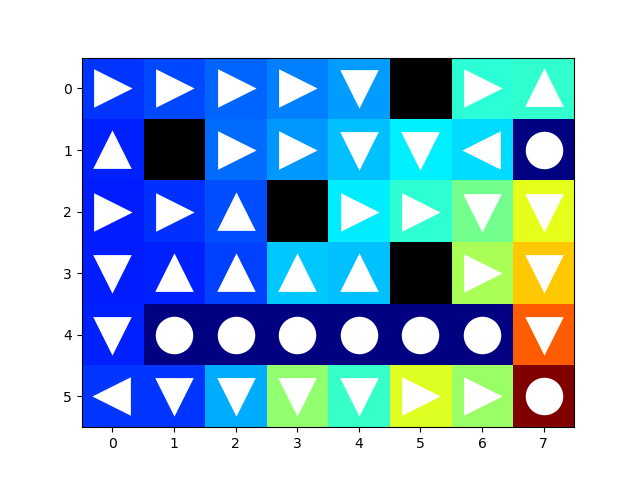
\includegraphics[scale=0.5]{e=3.png} 
            \caption{epsilon=0.3} 
            \end{minipage}%  
            \begin{minipage}[t]{0.5\linewidth} 
            \centering 
            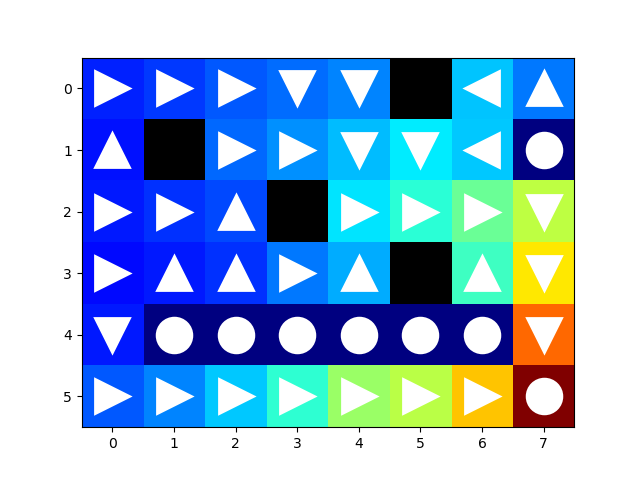
\includegraphics[scale=0.5]{ql_e_greedy.png} 
            \caption{epsilon=0.4} 
            \end{minipage}
            \\
            \centering 
            \begin{minipage}[t]{0.5\linewidth}
            \centering 
            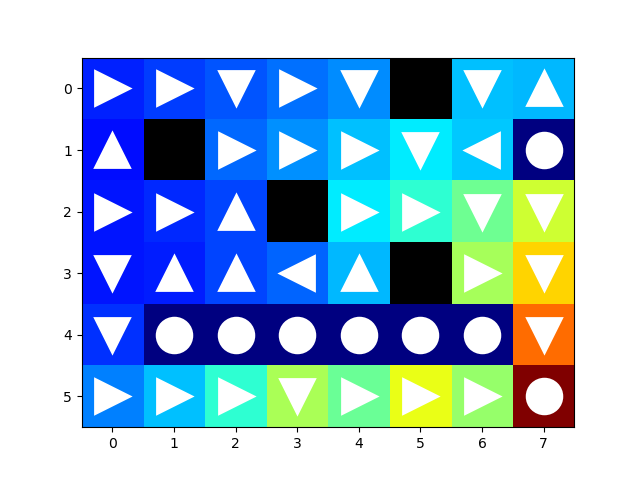
\includegraphics[scale=0.5]{e=5.png} 
            \caption{epsilon=0.5} 
            \end{minipage}%  
            \begin{minipage}[t]{0.5\linewidth} 
            \centering 
            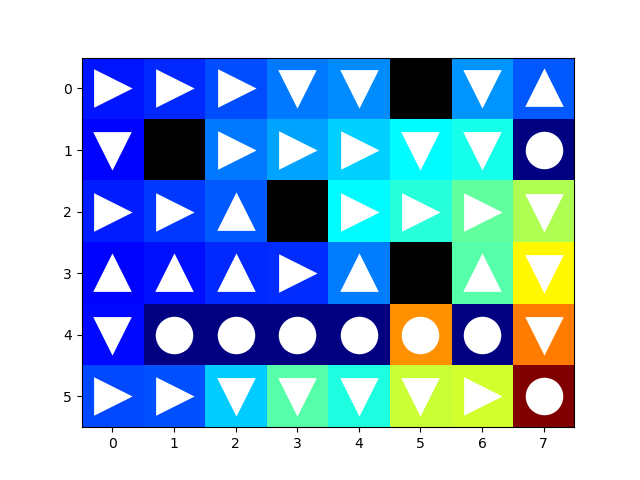
\includegraphics[scale=0.5]{e=6.png} 
            \caption{epsilon=0.6} 
            \end{minipage}
            \centering 
            \caption{Tuning epsilon} 
        \end{figure}
        \newpage
    \end{enumerate}
\subsection{More improvement}
From all the results above, I find a common problem that policy in the upper right 
is quite bad. However, I think it may not mean that the Q-learning algorithm goes wrong or 
the hyperparameters aren't tuned well. Because of the given position of initial state and goal state, the agent will 
hardly explore places on the upper right. To clarify it, just let the agent starts from different position when exploring. 
And here's the final policy.\\
\begin{figure}[htbp] 
    \centering 
    \begin{minipage}[t]{0.5\linewidth}
    \centering 
    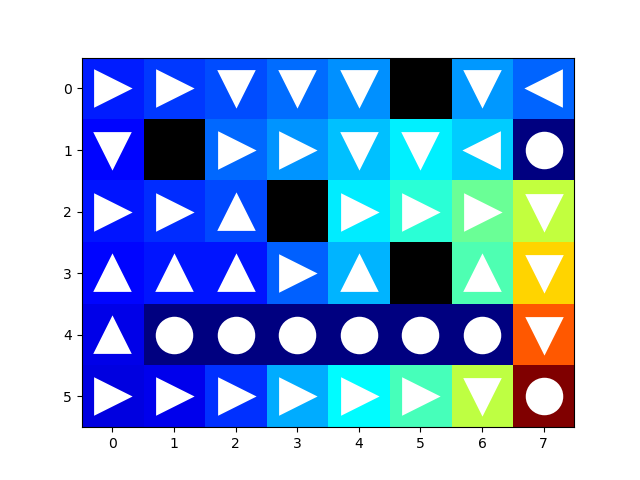
\includegraphics[scale=0.5]{_ql_explore.png} 
    %\caption{fig1} 
    \end{minipage}%  
    \begin{minipage}[t]{0.5\linewidth} 
    \centering 
    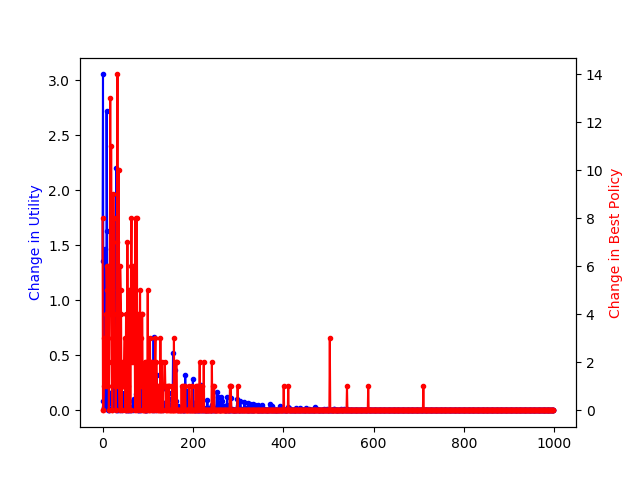
\includegraphics[scale=0.5]{_ql_explore_change.png} 
    %\caption{fig2} 
    \end{minipage}% 
    \centering 
    \caption{policy iteration} 
\end{figure}
\par It's a quite optimal result, and values and policies converge quite fast.
\newpage
\section{gym Pong-v0}
\subsection{The fundamental patten}
\begin{wrapfigure}{r}{3cm}
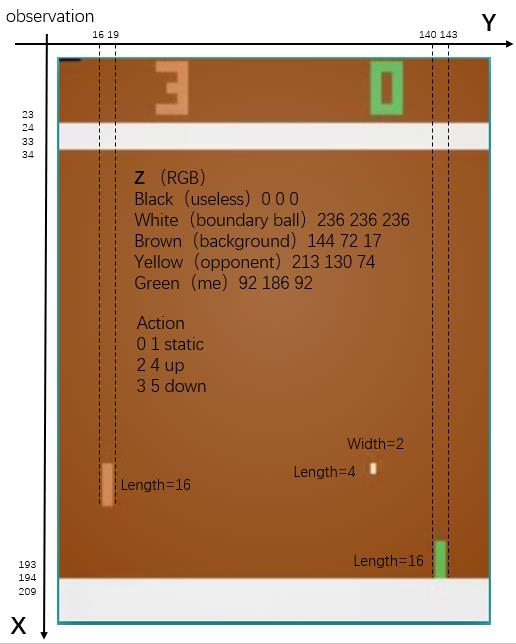
\includegraphics[width=3cm,clip]{pongv2.jpg}
\end{wrapfigure}
The main imformation we get from the game is a RGB image. 
It includes white ball, white walls, brown background, yellow and green board. 
We are to control the green board to play pong games. We can take 6 different actions to 
control our board and also change the ball's direction and speed when colliding it. We will lose 
scores when the opponent misses the ball, the program outputs a positive reward. When we get 21 reward, we will win the game. 
And vice versa. 
\subsection{Q-learning algorithm}
In the Q-learning algorithm, we do things as follows:
\begin{enumerate}
\item define the generalized state space from the observation
\item define the reward in some specific conditions
\item start with a simple guiding method to help it learn from scarch
\item save the learned Q and test it
\end{enumerate}
\subsubsection{state space}
From the RGB image, we can compute the positions of boards and ball. 
To make the state space smaller, we need to make it discrete using the vertical and horizontal distance between 
board and ball. Horizontally, I divide the 1st dimension $b$ of state space into 12 parts. If the ball's Y coordinate is larger than 
board's, which means the agent misses the ball, y equals to 0. And if ball is on the left of the background(ball's Y coordinate<60), b equals to 11. 
And the other 10 states are between the former 2 states. In vertical, which is quite important, I divide into 3 parts. If the ball's X axis is in the range of 
board, $a$ equals to 0. If the ball's X axis is smaller, $a$ equals to 1, and $a$ equals to 2 for larger similarly. At first, I also divide it into 10 states in vertical. 
But later I find no matter how long the vertical distance between board and ball, the agent should take the same action since the board's moving speed is stable. So finally, the state space is a $3*12$ array and Q is a $3*12*6$ array consequently.  
\subsubsection{reward}
Despite the game will give us reward periodically, but it is not 
precise enough to help the agent to learn. So I assume the agent will get a positive reward(r=2 indeed) when it catches the ball, and will get a negative reward(r=-5) when it misses the ball.
\subsubsection{guiding method}
If the agent begins to learn from scrach, it will take quite a lot of time to explore and therefore get a high regret. But if we use a simple sample to guide the agent, it will learn much faster. 
So I just write a simple PID control method and apply it at the first episode. 
\subsubsection{Testing}
After training, the learned Q will be saved as a .npy file. To test the performance. And I find it quite hard to get scores against the opponent though luckily the agent will get some scores.
And I've trained 8 models and the final model Q$\_$v7 gets the best performance after 50 episodes. I will submit these models as well so you can test it directly without training.
\subsubsection{Extra ideas}
I've got some ideas to improve the performance. But despite the deadline, I have no time to implement them.
\begin{enumerate}
    \item The Q-learn can be divide into 2 steps. First step is how to move the board to catch the ball and the second is how to hit the ball to make the opponent miss. 
    So we can record the last state and action when hit the ball. If the opponent miss the ball because the agent taked the right action to hit the ball, give that action a high reward in that state. 
    \item Using several observations nearby to get state, so the agent can get more information such as the ball's direction and speed. But the state space will get much larger and it will take more time to train the agent. 
\end{enumerate}
\end{document}